\documentclass{article}

\usepackage{ctex}
 
\usepackage{geometry}
\geometry{top=2cm, bottom=2cm, left=3cm, right=3cm}

\usepackage{multicol}
\usepackage{indentfirst}

\usepackage[colorlinks,linkcolor=blue]{hyperref}

\usepackage{amsfonts}

\usepackage{graphicx}

\usepackage{float}

\usepackage{appendix}



\title{Ubuntu对话语料:非结构化多轮对话系统数据集}
\author{Ryan Lowe, Nissan Pow, Iulian V.Serban and Joelle Pineau}
\date{}


\begin{document}
	\maketitle
	
	\begin{abstract}
		这篇文章介绍了Ubuntu对话语料。这个数据集包含了大约一百万个多轮对话,一共超过七百万个语句以及一亿个单词。这为基于可以利用大量未标记数据的神经语言模型构建对话管理器的研究提供了独特的资源。这个数据集既有对话状态跟踪挑战数据集的对话的多轮属性,也有来自微博服务(例如Twitter)的交互的非结构化特性。我们描述了两种适合分析这个数据集的神经网络结构,同时为挑选下一个最好的回复任务提供了基准性能。
	\end{abstract}

	\begin{multicols}{2}
	
	\section{介绍}
	计算机能够自然连贯的交流的能力长时间以来一直是人工智能(AI)的一个主要目标。在这篇文章中,我们讨论的问题是构建一个能够在各种话题进行一对一多轮交互的对话机器人。我们主要的目标是非结构化对话。在非结构话对话中,信息交换没有一种先验的逻辑表示。这不同于使用槽填充表示的结构化的对话任务。
	
	可以看到近些年来在AI的子领域——计算机视觉,语音识别,机器翻译——使用机器学习方法,具体来说是神经网络,已经取得了基础性的突破。然而这些大部分取得成功的方法,尤其是卷积神经网络以及递归神经网络,在很多年前就被提出了。可以将这些进步归功于三个主要因素:1) 公开的大型丰富的数据集,2) 足够的计算资源,3) 神经网络的新的训练方法,尤其是借助没有标记的数据。然而在对话系统的发展并没有相似的成功。我们认为这是由于缺少足够大的数据集,并希望通过提供一个新的用来研究多轮对话的大型语料来解决这个瓶颈。
	
	新的Ubuntu对话语料包含大约一百万个从Ubuntu聊天日志中提取出来的两个人的对话。Ubuntu聊天日志是用来为各种Ubuntu相关问题提供技术支持。这些对话平均每一个有八轮,最少的有3轮。所有对话都是文本的形式(不是录音的形式)。该数据集比结构话语料(例如那些对话状态跟踪挑战的数据集)大几个数量级。它和最近用来解决问答问题以及微博服务(例如Twitter)问题的数据集具有相同的规模,但是我们的数据集的对话包含的轮数更多,而且语句更长。更重要的是,因为它是基于特定领域的(技术支持),所以也可以用来研究基于特定应用的AI客户端,而不是通常的提前确定好一个目标的聊天机器人。
	
	除了这个语料,我们也提出了适合分析这个数据集的学习结构。从简单的 frequency-inverse document frequency(TF-IDF)方法,到更加复杂的递归神经网络(RNN)以及长短时记忆(LSTM)结构。我们用我们新的数据集在挑选下一个最好的回复的任务上为这些算法提供可基准性能。这个任务不需要任何人力标准。数据集将会公开发布\footnote{新版的数据集链接:\href{https://github.com/rkadlec/ubuntu-ranking-dataset-creator}{https://github.com/rkadlec/ubuntu-ranking-dataset-creator}},这些实验结果的代码\footnote{\href{http://github.com/npow/ubottu}{http://github.com/npow/ubottu}}也会公开。
		
	\section{相关工作}
		我们简要地回顾了现在的对话数据集,以及最近的一些对于结构化对话以及非结构化对话的学习结构。这并不是一个详尽的清单(由于空间限制),而是调查与我们贡献最相关的资源。图\ref{其他数据集统计}列出了讨论的数据集。
		
				
		\subsection{对话数据集}
		Switchboard数据集和对话状态跟踪挑战(DSTC)数据集已经被用来训练和验证用于交互信息检索的对话管理系统。问题通常被建模为一个槽填充的任务,客户端在对话的过程中想要预测这个用户的目的。尽管这些数据集和现在用来训练神经网络的数据集来比是非常小的,但是他们对于结构话的对话来说是非常重要的资源,而且已经推动了这个领域的主要的发展。
		
		最近一个从Twitter\footnote{\href{https://twitter.com/}{https://twitter.com/}}提取出来的数据集被用来训练非结构化对话系统。Ritter等人收集了一百三十万个对话。通过使用A-B-A三元组的形式,这些对话能够被用来作为更长的文本。Shang等人使用了一个相似的叫做微博\footnote{\href{http://www.weibo.com/}{http://www.weibo.com/}}的中国网站。然而据我们所知,这些数据集尚未公开,而且此类微博服务的回复格式可能并不像在一个聊天室中人和人之间的那种连续消息流的自然对话一样。事实上,Ritter等人估计了大概只有37\%的Twitter上的内容具有自然对话的特性,而且他们收集的69\%的数据的交互长度只有2。我们假设聊天室的消息风格和人类之间的对话更加接近,而不是微博客网站或者基于论坛的网站(Reddit)。
		
		部分Ubuntu聊天日志以前已经被作为一个叫做Ubuntu Chat Corpus的数据集。但是这个数据集保留了多个参与者的结构,因此不太适合调查传统的两个人的对话。
		
		和我们的贡献相关性比较弱的是问答(question-answer)系统。现在有各种问答对的数据集,但是这些数据集的交互长度比我们想要研究的要短的多。
		
		\subsection{学习结构}
		
		大部分的以前的对话研究聚焦于结构化的槽填充(slot-filling)任务。各种方法被提出,但是使用最近的神经网络模型的方法不是很多。	一个值得注意的例外是Henderson等人的工作,提出了一种用去噪自动编码器的RNN结构用来解决DSTC的三域问题。
		
		在非结构化的对话的研究中,最近Ritter等人提出在Twitter数据集上基于统计机器翻译提出了回复生成模型。这种方法的性能超过了以前的信息提取(最近邻)方法。这种想法被Sordoni等人进一步的拓展,使用了一种和RNN的编解码器模型相类似的结构。这种方法在Twitter的A-B-A数据集上使用BLEU值(一种机器翻译的标准)来测量时性能不是很好,但是比Ritter等人的模型性能要好一些。他们的结果也经过了人工评判。一个相似的编解码结构也被提出。这种模型使用一个RNN来将输入编码为一个向量表示,然后另一个RNN来将这个向量表示通过一次生成一个单词的形式生成回复。这种方法页经过了人工评判。总体来说,这些模型表现出对于交互系统来说神经网络的潜力,但是到目前位置,这些都只限于非常短的对话。
		
		\begin{figure*}[htbp]
			\centering
			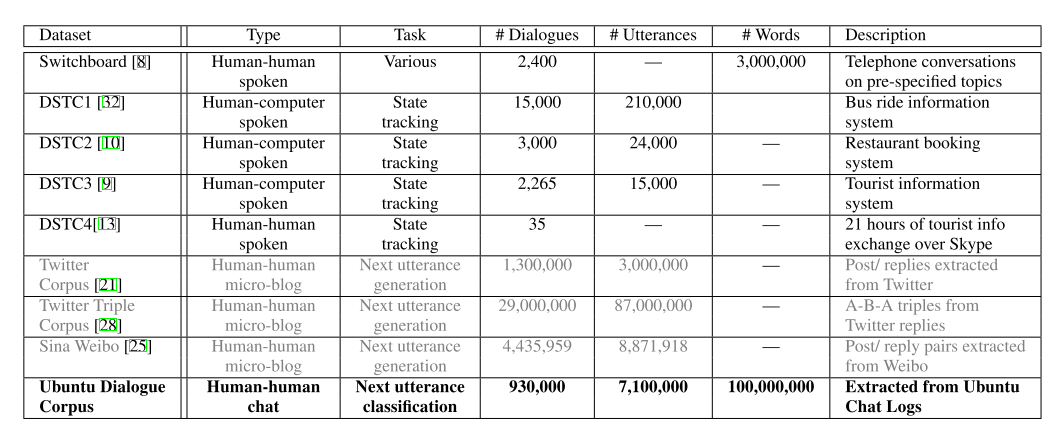
\includegraphics[scale=0.4]{./images/table1.png}
			\caption{结构化以及非结构化的可用于对话系统的数据集。灰色的数据集未公开,最后一行是我们的数据集。}
			\label{其他数据集统计}
		\end{figure*}
		
		
	\section{Ubuntu 对话语料}
	
	我们寻找对于研究对话系统的具有以下属性的大型数据集:
	\begin{itemize}
		\item 双人对话,不同于多人聊天。
		\item 数量大:对于AI领域使用神经网络的方法典型的数据集大小是 $10^5 - 10^6$。
		\item 对于各种轮数都有很多对话。
		\item 特殊的任务领域,不同于聊天机器人。
	\end{itemize}

	这篇文章提出的Ubuntu 对话语料满足上面的所有要求。
	
		\subsection{Ubuntu 聊天日志}
		Ubuntu聊天日志是指在Freenode Internet Relay Chat(IRC)网站上的与Ubuntu相关的聊天室收集的聊天日志。这个网站允许很多人同时实时聊天。每一个聊天室有一个特定的主题,而且每一个聊天室的人能够看到所有的聊天信息。很多这些聊天室是为了获得关于Ubuntu的各种问题的技术支持。
		
		由于每个聊天室的内容都经过审核,所以大部分的聊天都遵循着相似的模式。一个新的用户加入聊天室,询问一个关于Ubuntu的问题。然后另一个有经验的用户先打出这个问问题的用户的名字,然后回复一个可能行的解决方案。在回复之前需要先强调自己回复的是谁,这可以避免冲突。在一个聊天室中,可以同时存在1到20个对话。在大部分的聊天室中,一个时间点几乎不会只有一个对话。这位我们提取两个人之间的对话带来了麻烦。一对用户之间的对话在问题被解决之后就会停止,但是偶尔还会有人继续讨论和Ubuntu不相关的问题。
		
		尽管聊天室中的信息流是来自多个用户的,但是我们可以通过严禁的结构来提取出用户之间的对话。图\ref{Ubuntu聊天日志转聊天语料} 展示了一个 \# Ubuntu聊天室的对话以及从中提取出来的用户之间的对话。从中可以看出人们在发送他们的回复的时候通常会先说明自己的回复是给谁的。(我们所有的回复和一开始提出的问题称作‘utterances’)。例如,显然用户‘Taru’和‘kuja’正在进行对话,用户‘Old’和‘bur[n]er’也在进行对话。而用户‘\_pm’正在提问题,‘LiveCD’可能正在详细阐述之前的评论。
		
		\subsection{数据集生成}
		
		为了生成Ubuntu对话语料,首先需要一种方法从聊天室中的多人对话提取出双人对话。第一步是将每一条消息分成四元组(time,sender,recipient, utterance)。有了这些四元组,能够直接将发送者和接受者匹配的四元组分组。虽然很容易将时间和发送者提取出来,到那时找到这条消息的接受者却并不都很容易。
		
		\subsubsection{接收者识别}
		大多数情况下接受者是这句话的第一个单词,但是有时候接收者在这句话的最后,或者在提问题的时候根本就不存在。还有很多人选择很常见的英文单词作为名字,如‘the’或者‘stop’,这通常会导致很多误报。为了解决这个问题,我们从当天和之前的对话中建立了一个用户名词典,然后匹配每句话的第一个单词和这个词典中的元素。如果匹配上了,而且这个单词不是一个非常普通的英语单词\footnote{我们使用GNU Aspell 拼写检查词典。},那么就认为这个用户是这条消息的接收者。如果没有匹配上,那么就认为这条消息是一个问题,接收者为空。
		
	
		\subsubsection{语句生成}
		
		对话提取算法通过从第一个回复在三分钟的时间帧长中往回寻找这个回复回答的问题。第一条回复通过接收者名字来判断。最开始的问题是这个第一个回复标记的接受者的最近的发言。
		
		所有没有被判断为第一个回复或者问题的发言都被丢弃,如果一个问题没有任何回复也会被丢弃。如果一个超过五轮的对话,其中一个用户发言超过80\% ,那么我们也把它丢弃,因为这些并不能够代表典型的真实聊天对话。最后我们仅仅保留超过三轮的对话,来鼓励对长时间依赖关系进行建模。
		
		有些时候一个用户没有指明这句话的接受者,如图\ref{没有指明接收者}所示。为了解决这个问题,我们检查每个用户是否在他的谈话期间和别人进行交谈。如果没有,那么就将所有的没有标明接收者的发言添加到这个对话中。图\ref{没有指明接收者}是一个这样的例子。注意到我们将一个人的连续对话拼接到了一起。
		
		\begin{figure}[H]
			\centering
			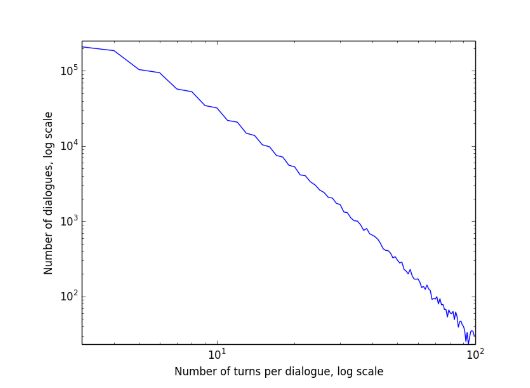
\includegraphics[scale=0.4]{./images/figure1.png}
			\caption{给定轮数的对话的数量。两个坐标轴都是对数坐标。}
			\label{数量与轮数的关系}
		\end{figure}
		
		\begin{table}[H]
			\centering
			\begin{tabular}{|p{4cm}|c|}
				\hline
				\centering \# dialogue(human-human) & 930,000 \\
				\hline
				\centering \# utterances(in total) & 7,100,000\\
				\hline
				\centering	\# words(in total) & 100,000,000\\
				\hline
			\centering 	Min.\#turns per dialogue & 3 \\
				\hline
			\centering 	Avg.\#turns per dialogues & 7.71 \\
				\hline
			\centering 	Avg.\#words per utterance & 10.34 \\
				\hline
			\centering 	Median conversation length(min) & 6 \\
				\hline
			\end{tabular}
			\caption{Ubuntu 对话语料的属性}
			\label{数据集属性}
		\end{table}
		我们没有对这个发布的Ubuntu对话语料数据集进行任何其他的预处理。然而对于大部分NLP系统预处理是必须的,同样我们的后面的分析也进行了预处理。(见第四部分)
		
		\subsubsection{特殊情况以及局限性}
		
		通常一个用户会提出一个问题然后很多人会对这个问题进行不同的回答。在这种情况下,第一个用户和每一个回复的用户之间都被提取出一个独立的对话。让同一个问题在各种对话中重复出现有坏的副作用。但是这种情况的数量和整个数据集规模比起来是非常小的。
		
		另一个需要注意的问题是发言的时间是没有被考虑的。虽然两个人的对话持续数小时甚至数天,我们任把它看做一个对话。但是现实中这种对话是很少的。我们将发言时间也保留在了数据集中使得其他人能够利用这些信息。
		
		\subsection{数据集统计信息}
		
		表\ref{数据集属性}总结了Ubuntu对话语料的统计信息。一个最重要的属性是它的大小。这对于基于神经网络的方法研究构建对话管理器是十分重要的。另一个重要的统计特性是这些对话的轮数。轮数的分布见图1。可以看出对话的数量和对话的轮数满足某种近似幂律关系。
		
		\subsection{生成测试集}
		
		我们从Ubuntu 对话数据集中随机挑选了2\%作为测试集,用来评估回复挑选算法。与剩余的语料相比,测试集被进一步预处理了。每一个对话会提取出一对(context, response, flag)三元组。flag是一个布尔值变量,用来标记在给定上下文的情况下,当前响应是否是真正的下一个语句。response 是一个我们希望正确识别的目标语句。context包含这个回复语句之前出现在对话当中的所有语句。我们生成了一对三元组,其中一个三元组包含正确的回答(对话中真正的下一条语句),另一个三元组包含在测试集中随机挑选的一个错误回答。第一种情况的flag值为1,第二种情况的flag值为0。表\ref{测试集样例}展示了一对三元组的例子。为了使任务变得更加困难,可以将一对回复拓展为错误回答更多的情况(所有这些错误回复的flag都是0)。在下面的实验中,我们考虑了1个错误回复和10个错误回复两种情况。
		
		\begin{table}[H]
			\centering
			\begin{tabular}{|p{3cm}|p{2.5cm}|c|}
			\hline
			\centering Context & \centering Response & Flag \\
			\hline
			\centering well,can I move the drives?\_EOS\_ah not like that & I guess I could just get an enclosure and copy via USB & 1 \\
			\hline
			well,can I move the drives?\_EOS\_ah not like that & you can use "ps ax” and "kill (PID \#)" & 0 \\
			\hline	
			\end{tabular}
			\caption{测试集样例。‘\_EOS\_’表示上下文中一个语句的结束。}
			\label{测试集样例}
		\end{table}
		
		因为我们希望学习预测一个对话的任意部分,而不是对话的最后的陈述,所以我们考虑对我们的测试集进行各种上下文分割。上下文的大小使用下面的公式进行随机的决定。
		
		$$ c = min(t-1, n-1) , $$
		\quad where $ n = \frac{10C}{\eta} + 2 , \eta \sim  Unif(C/2. 10C)$
		
		这里,$C$ 表示最大的上下文大小,我们设置为20。最后一项表示最小的上下文大小,我们设置为2。参数$t$表示当前对话真正的长度(所以有$c \le t -1 $ 这个限制条件),$n$是对应于随机采样上下文长度的随机数。
		
		实际中,这会使得短的测试对话产生短的上下文,长的对话通常分解成短的或者中等长度的上下文。偶尔会有10轮或者更多轮的长的上下文。
		
		\subsection{评估方法}
		
		我们研究的问题是最好的回复挑选。可以使用3.4部分的方法来预处理数据,而不需要任何人工标注。该分类任务是对先前应用于对话数据集的召回和精确度量的改编。
		
		一类用于语言任务的度量方法是Recall@k(下面标注为R@1 R@2, R@5)。客户端挑选$k$个最可能的回复,如果真实的回复在这写$k$个候选项当中时,就判定为正确。只有R@1和二分类任务相关。
		
		虽然一个模型在挑选下一个回复的问题上表现很好,但是这并不意味着在下一个回复的生成上也会表现的很好。我们认为一个模型在分类任务上性能的提升最终会促进在生成任务上性能的提升。关于这一点第六部分有更多的讨论。
		
	\section{非结构化对话的学习结构}
	
	为了证明我们的数据集对于研究神经网络方式搭建对话管理器具有重要的价值,我们对于两种学习算法提供了性能基准。方法包括:TF-IDF,递归神经网络(RNN),以及长短时记忆(LSTM)。在使用每种方法之前,我们使用NLTK\footnote{\href{www.nltk.org}{www.nltk.org}}库和Twitter 分词器\footnote{\href{http://www.ark.cs.cmu.edu/TweetNLP/}{http://www.ark.cs.cmu.edu/TweetNLP/}}来解析每一个语句。我们为各种单词类别产生通用的标签,如人名,位置,组织,URL以及系统路径。
	
	为了训练RNN和LSTM结构,我们利用3.4部分的方法处理了整个训练集,提取出(context, response, flag)三元组。对于测试集,我们不随机选取上下文的长度,而是将每一个语句作为一个回复(从第三句开始),然后把前面的语句作为上下文。所以一个10轮的对话能够生成8个训练样本。由于存在重叠,让门显然是不独立的。但是考虑到数据集的规模,这不是一个很大的问题(在训练的时候随机混洗)。错误的回复在剩下的训练集中随机挑选。
	
		\subsection{TF-IDF}
		Term frequency-inverse document frequency 是一个用于估计一个单词对于一个文本的重要性的统计特征。
		这种技术通常用于文本分类以及信息提取。‘term-frequency’是一个文本中一个单词出现的频率。‘inverse document frequency’衡量了一个单次在这个语料中其他文本出现的频率。最终的得分是这两项的乘积:
		$$tfidf(w,d,D) = f(w,d) \times \log \frac{N}{|d \in D:w \in d|}$$
		其中$f(w,d)$衡量了单词$w$在上下文$d$中出现的次数,$N$是所有对话的数量,分母代表出现单词$w$的对话的数目。
		
		对于分类任务,首先从上下文和每一个候选的回复中计算出TF-IDF向量。然后从这些候选的回复向量中,选择和上下文向量具有最大余弦相似度的最为输出。对于Recall@k,前k个最高的最为输出。
		
		\subsection{RNN}
		
		递归神经网络是神经网络的变种,允许在神经单元之间进行时延有向循环。这使的网络具有内部状态$h_t$,能够对时间依赖数据进行建模。内部状态在每一个时间步都会用当前观测的输入$x_t$以及前一时刻的隐藏状态$h_{t-1}$的函数来进行更新。$W_x$和$W_h$是连接输入和隐藏状态的矩阵。
		$$h_t = f(W_h h_{t-1} + W_x x_t)$$
		
		
		\begin{figure}[H]
			\centering
			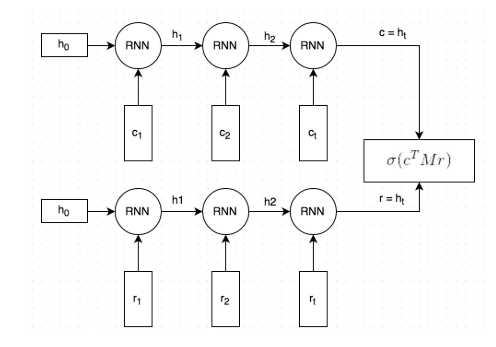
\includegraphics[scale=0.4]{./images/figure2.png}
			\caption{我们模型图示。两个RNN有相同的权重。$c,r$是两个RNN最后的隐藏状态。$c_i,r_i$表示上下文和回复的单词向量,$i < t $。我们的上下文最大值$t = 160 $。}
			\label{模型示意图}
		\end{figure}
		
		图\ref{模型示意图}是RNN的一个图示。RNN已经称为现在神经网络语言模型的主要构建模块。第一个RNN被用来编码上下文,第二个RNN用来通过使用束搜索(beam-search)来生成回复。第二个RNN的隐藏状态的初始值使用第一个RNN的最终的隐藏状态。在我们的工作中,我们考虑的问题是挑选回复,而不是生成回复。
		
		我们使用一种相似的包含两个RNN的网络来生成上下文和回复的嵌入。这两个网络的权重是一样的。给定上下文和回复,我们先一个时间步输入一个词嵌入到相应的网络中,然后得到对应的上下文和回复的嵌入$c,r \in \mathbb{R}^d$。词嵌入使用预训练的向量(Common Crawl)初始化,在训练的时候进行微调。RNN的隐藏状态每一步都会进行更新,最后的隐藏状态代表了整个输入的语句。使用两个RNN最终的状态,我们能够计算这两者是一对的概率
		$$p(flag = 1 | c,r,M) = \sigma ( c^T M r + b)$$
		
		偏置$b$和矩阵$M \in  \mathbb{R}^{d \times d}$是可学习的参数。这可以看做一种生成的方式。给定回复,我们通过使用$c' = Mr$来生成上下文然后通过内积测量它和真正上下文的相似度。然后通过一个sigmoid函数变成概率。模型通过最小化所有标记对的交叉熵来优化参数。
		$$L = -\sum_n{\log p(flag_n | c_n, r_n, M)} + \frac{\lambda}{2} ||\theta||_F^2$$
		
		$||\theta||_F^2$是$\theta = \{M ,b \}$的 Frobenius范数。在我们的实验中,为了方便将$\lambda$设为0。
		
		训练中,我们从训练集中随机挑选比例为1:1的正样本和负样本。RNN是具有一个50个神经元的隐藏层。$W_h$矩阵使用正则权重进行初始化,$W_x$使用-0.01-0.01之间均匀分布的随机数进行初始化。使用gradients clipped为10的Adam作为我们的优化器。我们发现权重初始化和优化器的选择对于训练RNN是非常重要的。
		
		\subsection{LSTM}
		
		除了RNN模型,我们将隐藏层单元设置为LSTM并使用了相同的结构。LSTM主要是用来建模长时间的依赖。这通过使用一系列的门来决定是否一个新的输入需要被记住或者被遗忘或者用来作为输出。可以将错误信号无限期地反馈到LSTM单元的门中。这能够解决标准RNN中误差以指数速率上升或下降带来的梯度消失和梯度爆炸问题。训练过程中,使用具有200个神经元的隐藏层。超参数配置(包括隐藏层个数)优化对于RNNs和LSTMs是独立的,通过使用从训练集中选取的交叉验证集。
	\section{实验结果}
	
	表\ref{实验结果}列出了TF-IDF,RNN和LSTM模型的实验结果。模型利用1(1 in 2)和9(1 in 10)个错误样本来进行评测。
	
	\begin{table}[H]
		\centering
		\begin{tabular}{|c|c|c|c|}
			\hline
			Method & TF-IDF & RNN & LSTM \\
			\hline
			1 in 2 R@1 & 65.9\% & 76.8\%  & \bfseries 87.8\% \\
			\hline
			1 in 10 R@1 & 41.0\% & 40.3\% & \bfseries 60.4\% \\
			\hline
			1 in 10 R@2 & 54.5\%  & 54.7\% & \bfseries 74.5\% \\
			\hline
			1 in 10 R@5 & 70.8\% & 81.9\% &  \bfseries 92.6\% \\
			\hline  
		\end{tabular}
		\caption{三种算法的结果。}
		\label{实验结果}
	\end{table}
	
	可以观察到LSTM在所有的评价指标上均优于TF-IDF以及RNN。有趣的是TF-IDF对于十选一在Recall@1上的性能比RNN要好。这可能是因为RNN处理长文本的能力有限,而这一缺点能够被LSTM克服。表\ref{LSTM例子}展示了LSTM分类正确的一个例子。
	
	在图\ref{LSTM性能提高}中我们也画出了随着训练数据的增加LSTM性能的增加曲线。这证实了有一个大的训练数据集的重要性。
	
	\begin{table}[H]
		\centering
		\begin{tabular}{|p{6cm}|}
			\hline
			Context \\
			\hline
			“any apache hax around ?i just delete all of \_path\_ - which package provides it?”, “reconfiguring apache do n't solve it ?” \\
			\hline
		\end{tabular}
	
		\begin{tabular}{|p{5cm}|c|}
			\hline
			\centering Ranked Response & Flag \\
			\hline
			\centering 1.“does n't seem to, no” & 1 \\
			\hline
			\centering 2.“you can log in but not transfer files?” & 0 \\
			\hline
		\end{tabular}
		\caption{使用LSTM对回复排序的例子。}
		\label{LSTM例子}
	\end{table}
	
	\section{讨论}
	这篇文章主要引入了一个研究非结构化多轮对话系统的大型数据集,Ubuntu对话语料。我们描述了这个数据集的规模和属性。这种规模的数据集为使用丰富的神经网络模型来研究对话系统提供了可能。利用这个数据集来训练RNN和LSTM解决在对话中挑选下一个最好的回复的任务中,我们提出了初步的结果。使用LSTM的结构我们得到了更好的结果。这为未来的工作有很好的指向作用。
	
	\begin{figure}[H]
		\centering
		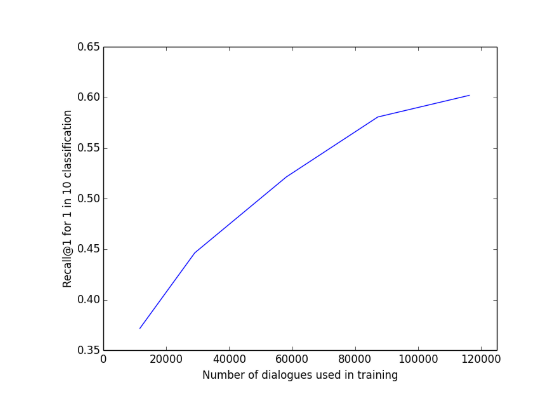
\includegraphics[scale=0.4]{./images/figure3.png}
		\caption{LSTM(200个隐藏单元),10选1的Recall@1 }
		\label{LSTM性能提高}
	\end{figure}
	\subsection{对话解构}
	
	我们用于对话结构的方法包含了一组规则。有很多更复杂的技术已经被提出了,如训练最大熵分类器来将话语聚类成单独的对话。但是我们并不是想要两个人之间的确切的对话,而是想检索合理的自然对话,所以本文中提到的启发式的方法已经足够了。
	
	\subsection{改变测试集难度}
	挑选回复任务一个有趣的性质是能够以一种可控的方式改变任务的难度。我们通过将错误回复从1个变成9个同时变化召回率k参数来演示了这一点。未来,我们将会考虑和真实回复相似的错误回复(用余弦相似度表示)。和单纯挑选与上下文具有最多相同单词的方法如TF-IDF相比,在这个更加困难的任务上表现好的模型也应该能够捕获句子的更细颗粒的语义含义。
	
	\subsection{状态跟踪和语句生成}
	
	这里描述的工作聚焦于回复挑选的任务。这可以看做一种处于槽填充和语句生成中间的情况。在槽填充中,候选输出(状态)集合是一种通过知识工程得到的先验信息,这和我们工作中的回复集合很相似。当候选响应集合和数据集的大小相近的时候(所有曾经记录的语句),那么就和生成回复的情况很接近了。
	
	不直接生成回复还有一些原因。首先,对于目前的算法而言还不能够很好地生成好的结果,最好是能够解决我们可以取得进展的指标。其次,在回复生成方面,我们还没有能够找到一种比较好的评价机制。一个可选的方法是机器翻译领域的BLEU值或者METEOR值。但是由于潜在可能的有意义的回复空间非常大,所以使用BLEU值来评价对话系统会给出非常低的分数。而且,因为BLEU值是使用N-grams来计算的,所以对于那些和真实的下一个语句相同词不是很多但是也合理的回复,它会给非常低的分数。
	
	或者,可以通过比较生成的语句和真实的句子在嵌入(或者语义)空间中的距离来判断两者之间的距离。然而,不同的模型不可避免地需要使用不同的嵌入,因此需要使用标准化的嵌入来评估。现在还未创建这种标准化的嵌入。
	
	还有一种方法是通过使用人力来为生成的回复打分,但是这总方法是一种非常耗时而且不切实际的。
	
	总而言之,虽然现在的语言模型可能已经超出了使用槽填充作为度量标准,我们现在仍然没办法以一种标准化的有意义的而且廉价的方式来测量他们生成下一个语句的能力。这使我们暂时使用语句挑选作为一个有用的指标。
	
		
	\end{multicols}
	\bibliographystyle{plain} \bibliography{reference}
	
	\newpage
	\appendix
	\appendixpage
	\section{对话摘抄}

	\begin{figure}[H]
		\centering
		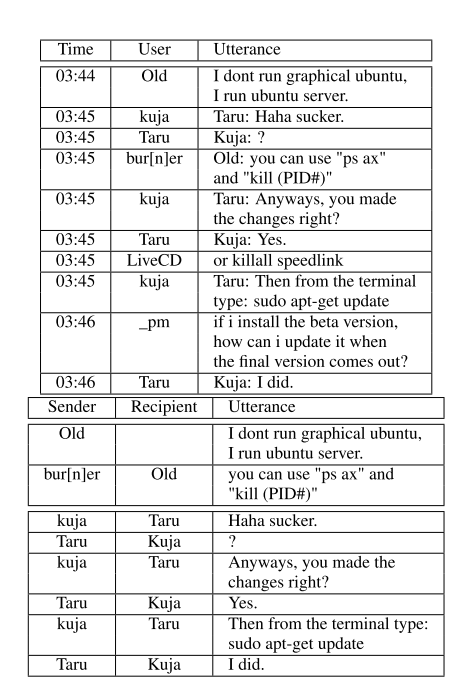
\includegraphics[scale=0.4]{./images/figure4.png}
		\caption{Ubuntu 聊天室聊天日志(top), Ubuntu对话语料(bottom)}
		\label{Ubuntu聊天日志转聊天语料}
	\end{figure}
	
	\begin{figure}[H]
		\centering
		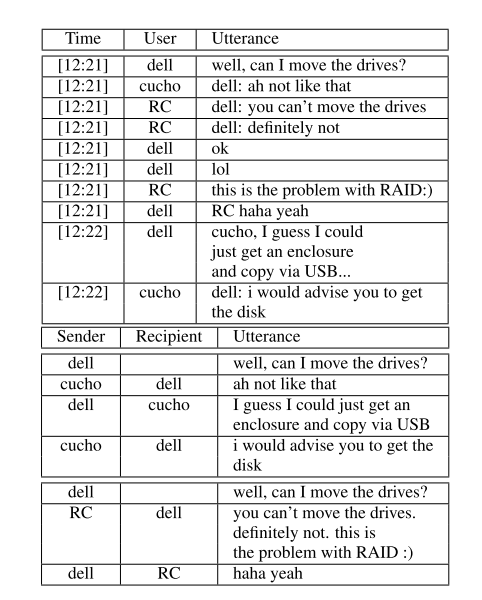
\includegraphics[scale=0.4]{./images/figure5.png}
		\caption{没有指明接收者的例子。}
		\label{没有指明接收者}
	\end{figure}
	
	
	
\end{document}